% Section 3 - Basic Communication
% Roberto Masocco <roberto.masocco@uniroma2.it>
% March 13, 2022

% ### Basic Communication ###
\section{Basic Communication}
\graphicspath{{figs/section3/}}

% --- ROS 2 Messages ---
\begin{frame}{ROS 2 Messages}
    \begin{block}{Definition of Message}
      A message is a \textbf{single DDS data packet} sent over a \textbf{topic}, from \textbf{publisher nodes} to \textbf{subscriber nodes}, with a specific \textbf{QoS policy}.
    \end{block}
    \begin{figure}
      \centering
      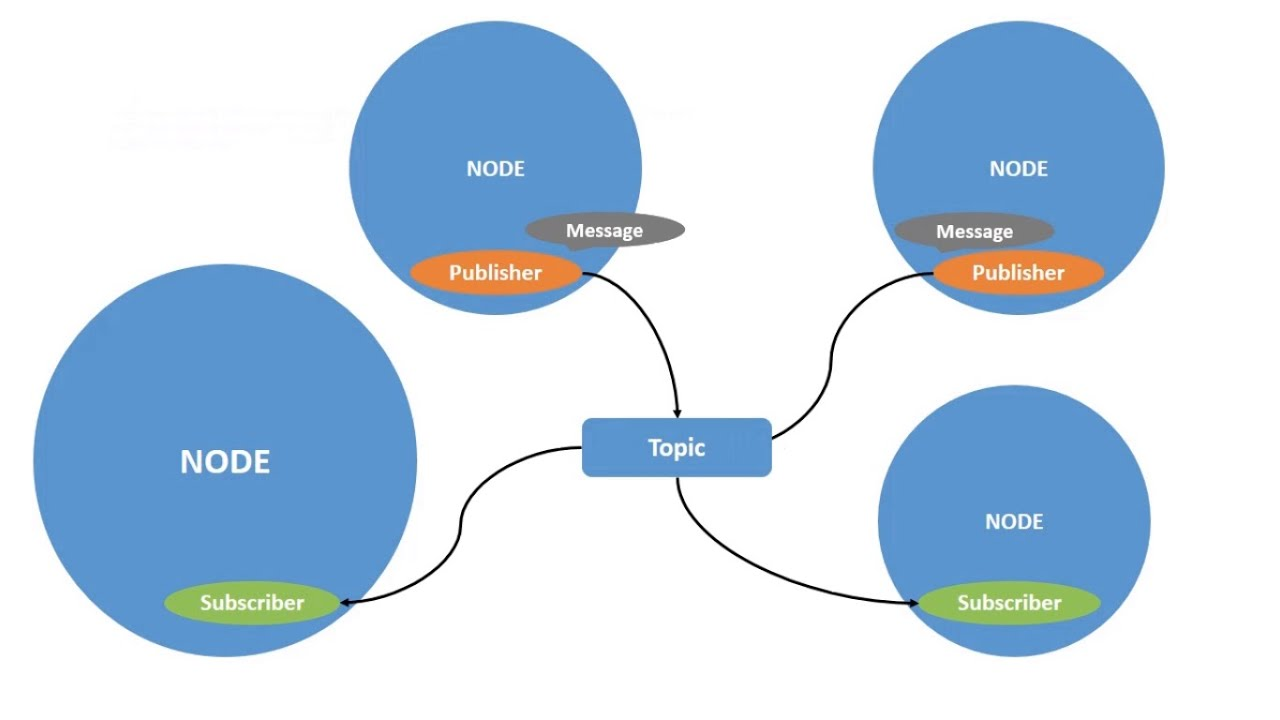
\includegraphics[scale=.19]{ros2Msg.jpg}
      \label{fig:msg}
      \caption{Example of a topic with multiple publisher and subscriber nodes}
    \end{figure}
\end{frame}

% --- Interface Files - Messages ---
\begin{frame}[fragile]{Interface Files - Messages}
Interface files format is specified by the DDS, with data types resolved to machine types according to the platform being used\footnote{\href{https://docs.ros.org/en/galactic/Concepts/About-ROS-Interfaces.html}{\color{blue}\underline{About ROS Interfaces}} (ROS 2 Galactic docs)}.\\
Things start very simply...

\begin{columns}
\column{.95\textwidth}
% Listing: std_msgs/msg/Int64 message definition
\begin{lstlisting}[language=ros2msg, caption=Definition of the \texttt{std\_msgs/msg/Int64} message]
int64 data
\end{lstlisting}

% Listing: std_msgs/msg/String message definition
\begin{lstlisting}[language=ros2msg, caption=Definition of the \texttt{std\_msgs/msg/String} message]
string data
\end{lstlisting}
\end{columns}

\end{frame}
\begin{frame}[fragile]{Interface Files - Messages}
... then escalate quickly!

\begin{columns}
\column{.95\textwidth}
% Listing: sensor_msgs/msg/Image
\begin{lstlisting}[language=ros2msg, caption=Definition of the \texttt{sensor\_msgs/msg/Image} composite message]
std_msgs/Header header

uint32 height
uint32 width

string encoding

uint8 is_bigendian
uint32 step
uint8[] data
\end{lstlisting}
\end{columns}

\end{frame}
\begin{frame}[fragile]{Interface Files - Messages}
Special values (i.e. constants) may be specified.

\begin{columns}
\column{.95\textwidth}
% Listing: message with constant
\begin{lstlisting}[language=ros2msg, caption=Definition of an example message with a constant value]
int64 MYNUM=1 # Must be of compatible type

int64 number
\end{lstlisting}
\end{columns}

They are not bound to any field and will appear as special selectable values in the generated C++/Python libraries.\\
ROS 2 adds its own guidelines\footnote{\href{https://github.com/IntelligentSystemsLabUTV/ros2-examples/blob/galactic/interfaces.md}{\color{blue}\underline{ros2-examples/interfaces.md}}}, and installed interfaces can be inspected with the \texttt{ros2 interface show} command.
\end{frame}

% --- Message Topics - Quality of Service ---
\begin{frame}{Message Topics - Quality of Service}
A \textbg{QoS policy}\footnote{\href{https://docs.ros.org/en/galactic/Concepts/About-Quality-of-Service-Settings.html}{\color{blue}\underline{About QoS Settings}} (ROS 2 Galactic docs)} for publishers/subscribers has the following attributes:
\begin{itemize}
  \item \textbg{History} (\emph{keep last N} or \emph{all})
  \item \textbg{Depth} (queue size \emph{N})
  \item \textbg{Reliability} (\emph{best-effort} or \emph{reliable}, default: reliable)
  \item \textbg{Durability} (publishers resend all messages to "late-joiners")
  \item Deadline
  \item \textbg{Lifespan} (message expiration date)
  \item Liveliness
  \item Lease Duration
\end{itemize}
Default \textbg{profiles} are available (e.g. \textbg{Sensor data}, \textbg{Service}...).
\end{frame}

% --- C++ Fundamentals ---
\begin{frame}[fragile]{C++ Fundamentals}
Dust off your C programming skills, then add:
\begin{block}{Object-Oriented Programming}
\begin{columns}
\column{.9\textwidth}
% Listing: C++ OOP example
\begin{lstlisting}[language=C++, caption=Example definition of a C++ class]
class MyClass : public ParentClass
{
public:
  MyClass();
  // ...
protected:
  // ...
private:
  // ...
};
\end{lstlisting}
\end{columns}
\end{block}
\end{frame}
\begin{frame}[fragile]{C++ Fundamentals}
\begin{block}{Namespaces}
Subdivision of the global namespace to avoid naming collisions between multiple libraries, resolved with the \texttt{::} operator.

\begin{columns}
\column{.9\textwidth}
% Listings: C++ namespaces usage example
\begin{lstlisting}[language=C++, caption=Example of namespaces usage]
MyLib::foo();
MyClass::foo();
// Completely different names for the compiler!
\end{lstlisting}
\end{columns}

Names may become very long, so usually they are hidden with \texttt{typedef}.
\end{block}
\end{frame}
\begin{frame}[fragile]{C++ Fundamentals}
\begin{block}{Templates}
Classes or functions whose implementation depends on some data type. When instantiated or called with a specific type, the corresponding code is generated by the compiler.

\begin{columns}
\column{.9\textwidth}
% Listings: C++ template objects example
\begin{lstlisting}[language=C++, caption=Example of objects of the template class \texttt{std::vector}]
std::vector<int> int_vector;
std::vector<double> double_vector;
\end{lstlisting}
\end{columns}

These too make names very long, so are usually typedef'd.
\end{block}
\end{frame}
\begin{frame}[fragile]{C++ Fundamentals}
\begin{block}{Shared Pointers}
A kind of \textbf{smart pointer} (there are also \texttt{unique} and \texttt{weak}) that also holds an \textbf{usage counter}, incremented by every function or object that is handling the pointer. \textbf{When the counter gets to zero, the pointer is reset and the memory which it points to is deallocated.}

\begin{columns}
\column{.9\textwidth}
% Listings: C++ shared pointer example
\begin{lstlisting}[language=C++, caption=Example of shared pointer creation]
{
  // A new scope starts here
  std::shared_ptr<rclcpp::Node> node =
    std::make_shared<rclcpp::Node>("my_node");
}
// The node pointer is reset here!
\end{lstlisting}
\end{columns}

Obviously that is a template class. ROS 2 heavily relies on them, and the \texttt{SharedPtr} alias is frequently defined.
\end{block}
\end{frame}

% --- Example: Topic Pub/Sub ---
\begin{frame}{Example: Topic Pub/Sub}
Go have a look at the \href{https://github.com/IntelligentSystemsLabUTV/ros2-examples/tree/galactic/src/topic_pubsub}{\color{blue}\underline{ros2-examples/src/topic\_pubsub}} package!
\end{frame}
